% !TEX program = lualatex
%!TEX TS-program = lualatex
\documentclass[12pt,a4paper]{article}

% --- JĘZYK I KODOWANIE ---
\usepackage{fontspec}
\setmainfont{Latin Modern Roman}
\setsansfont{Latin Modern Sans}
\setmonofont{Latin Modern Mono}
\usepackage[polish]{babel}

% --- USTAWIENIA STRONY ---
\usepackage[a4paper,margin=2.0cm]{geometry}
\usepackage{setspace}
\onehalfspacing
\setlength{\parindent}{0pt}
\setlength{\parskip}{6pt}

% --- TABELE, GRAFIKI, LINKI ---
\usepackage{booktabs}
\usepackage{longtable}
\usepackage{array}
\usepackage{graphicx}
\usepackage{float}
\usepackage{hyperref}
\usepackage{enumitem}
\graphicspath{{./}{screens/}{uml/}}
\hypersetup{
    colorlinks=true,
    linkcolor=black,
    urlcolor=blue
}
\urlstyle{same}

\begin{document}

\begin{center}
\begin{tabular}{ll}

\textbf{Tytuł projektu:} & Fortuna -- aplikacja dla klientów banku \\[6pt]
\textbf{Frontend:} & React, Vite, TypeScript, Redux Toolkit, TanStack Query \\[6pt]
\textbf{Backend:} & ASP.NET Core, .NET, Entity Framework Core \\[6pt]
\textbf{Bazy danych:} & SQL Server, osobna baza zapisu i baza odczytu \\[6pt]
\textbf{Architektura:} & Clean Architecture, DDD, CQRS, Outbox, Read Model \\[6pt]

\textbf{Autor 1:} & Jakub Wołczko\\
\textbf{Nr albumu:} & 70210 \\[6pt]

\textbf{Autor 2:} & Jakub Łaszuk \\
\textbf{Nr albumu:} & 72418 \\[6pt]

\textbf{Repozytorium:} & \href{https://github.com/jwolczko/Designing-multi-tier-business-applications}{GitHub -- Designing multi-tier business applications}

\end{tabular}
\end{center}

\newpage
\tableofcontents
\newpage

\section{Cel i zakres systemu}

Fortuna jest demonstracyjną aplikacją bankową dla klientów indywidualnych. System pozwala użytkownikowi założyć konto, zalogować się, obejrzeć dashboard produktów finansowych oraz wykonać przelew. Aplikacja została zaprojektowana jako system wielowarstwowy, w którym interfejs użytkownika komunikuje się z backendem przez REST API, a backend rozdziela model zapisu od modelu odczytu.

Zakres funkcjonalny obejmuje:
\begin{itemize}[nosep]
    \item stronę landing page z ofertą banku,
    \item rejestrację klienta oraz automatyczne utworzenie produktów startowych,
    \item logowanie z wykorzystaniem tokenu JWT,
    \item dashboard z podsumowaniem środków, listą produktów i historią zdarzeń,
    \item tworzenie przelewów własnych i zewnętrznych,
    \item symulację przelewu przychodzącego przez endpoint API,
    \item asynchroniczną aktualizację modelu odczytu przez mechanizm Outbox.
\end{itemize}

\section{Widoki aplikacji}

Frontend jest aplikacją SPA napisaną w React. Routing definiuje trzy ścieżki publiczne: landing page, logowanie i rejestrację oraz ścieżkę chronioną dashboardu. Po zalogowaniu token i identyfikator klienta są przechowywane po stronie klienta i używane do autoryzowanych wywołań API.

\subsection{Landing page}

Landing page prezentuje ofertę promocyjną banku, główną grafikę nawiązującą do Fortuny oraz kafle ofertowe. Z poziomu tego widoku użytkownik może przejść do rejestracji albo otworzyć modal logowania.

\begin{figure}[H]
    \centering
    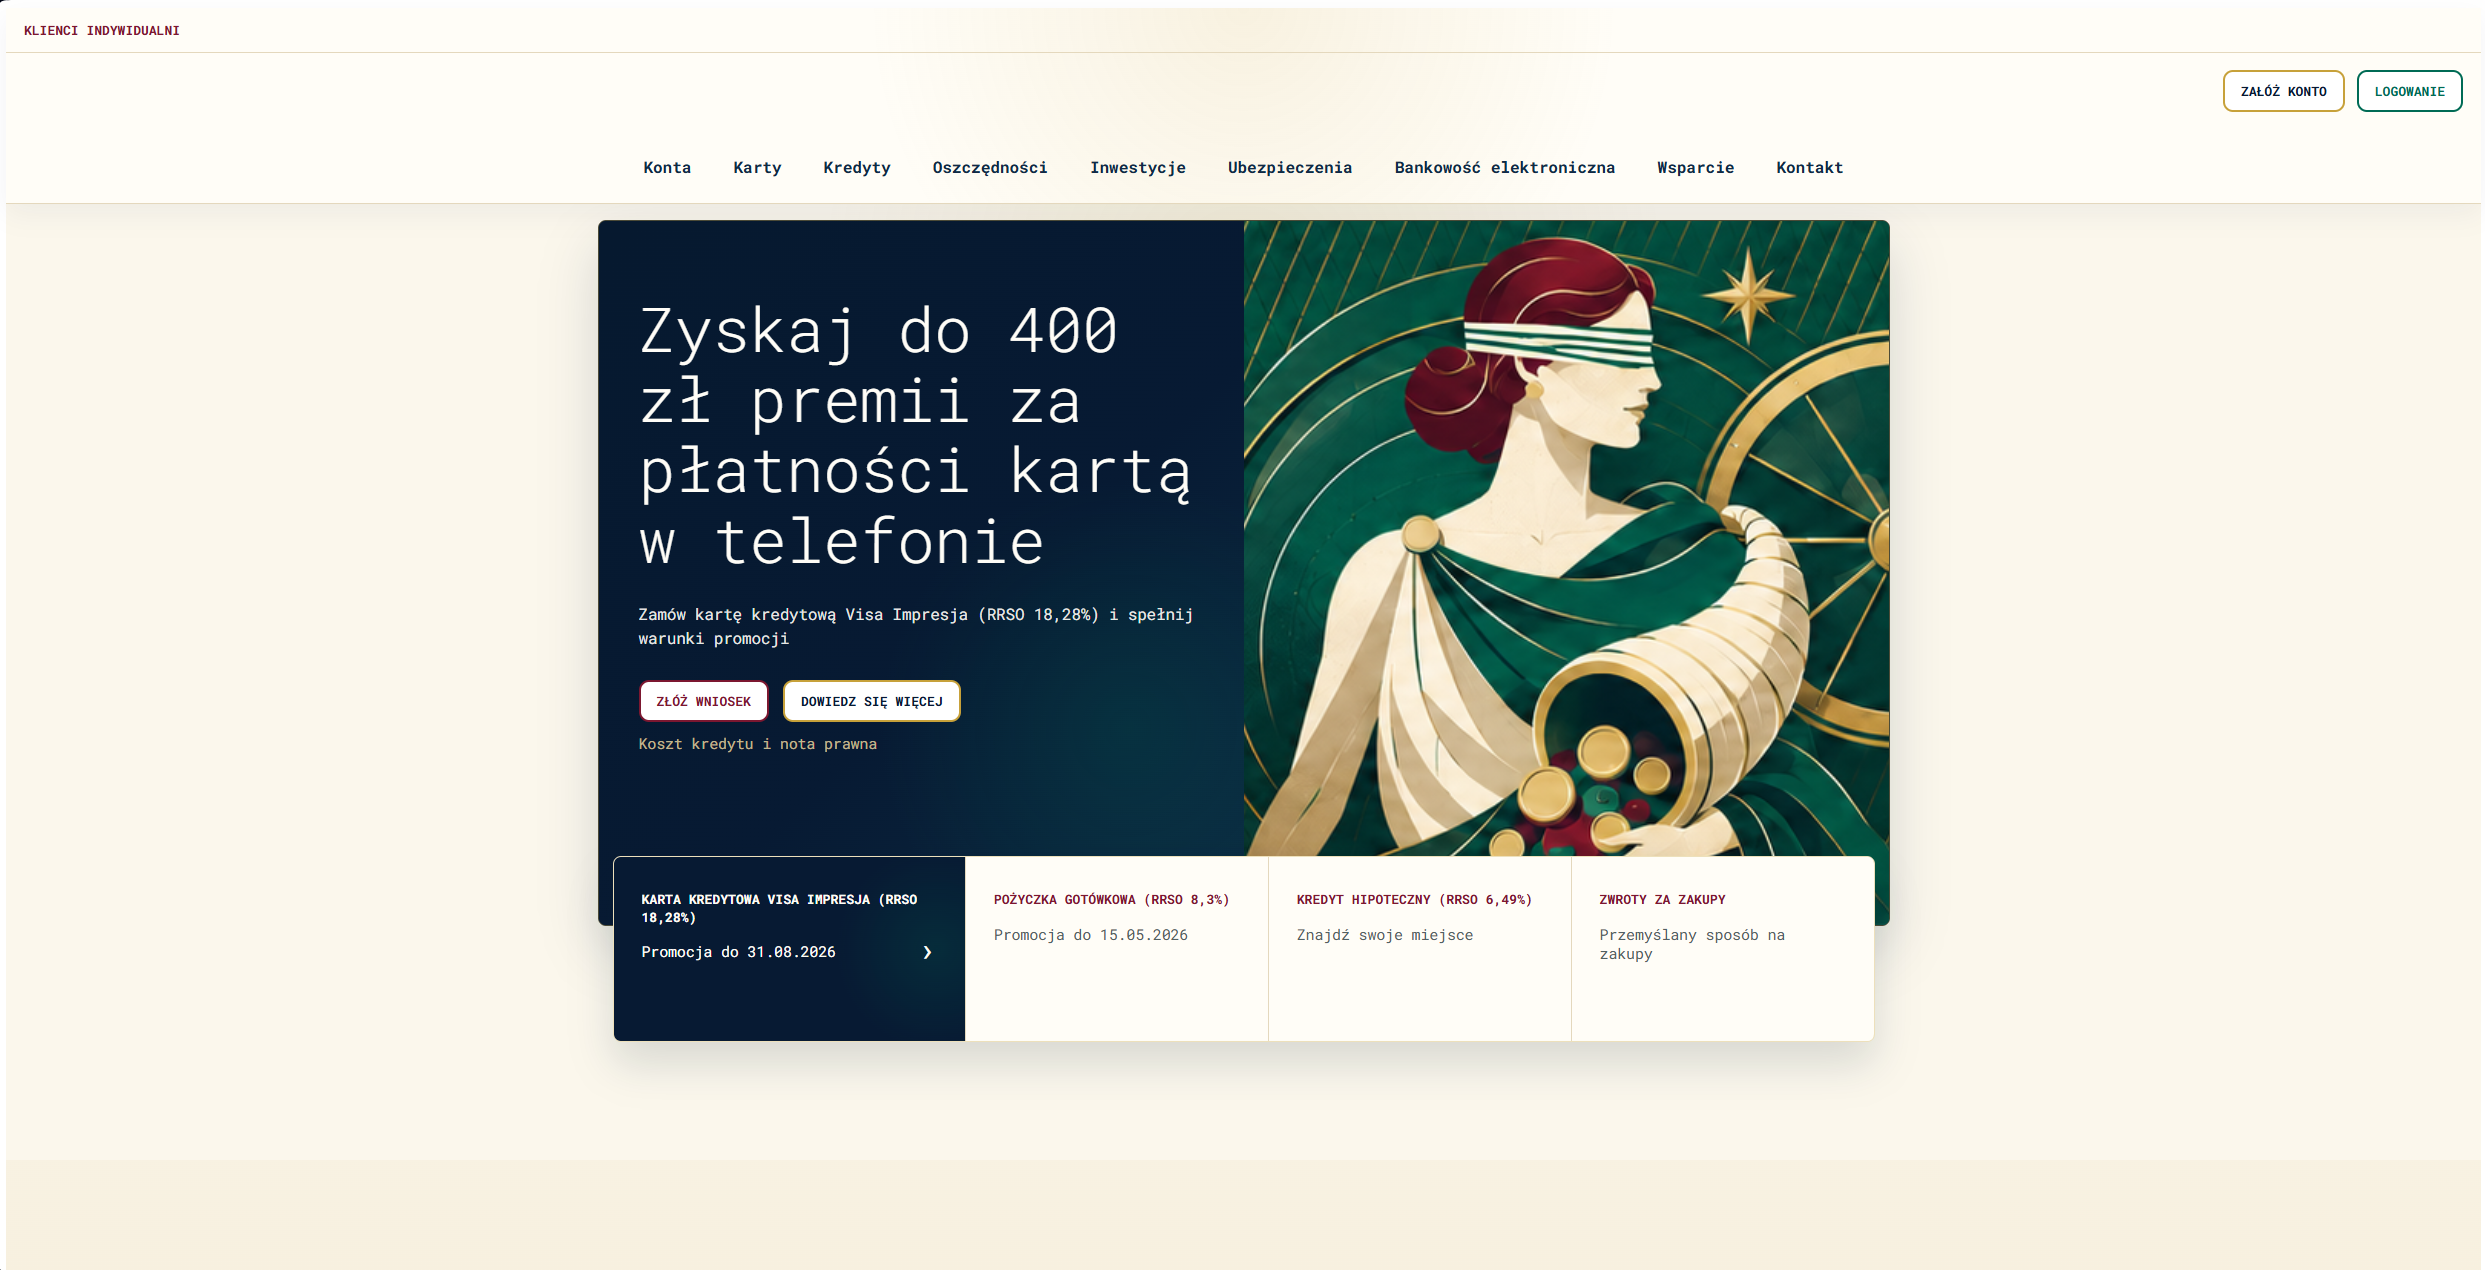
\includegraphics[width=0.95\textwidth]{landing_page.png}
    \caption{Landing page aplikacji Fortuna.}
\end{figure}

\subsection{Rejestracja użytkownika}

Formularz rejestracji zbiera imię, nazwisko, adres e-mail, hasło oraz typ klienta. Po przesłaniu formularza frontend wywołuje endpoint \texttt{POST /api/customers}. Backend waliduje dane, hashuje hasło i tworzy klienta razem z domyślnymi produktami.

\begin{figure}[H]
    \centering
    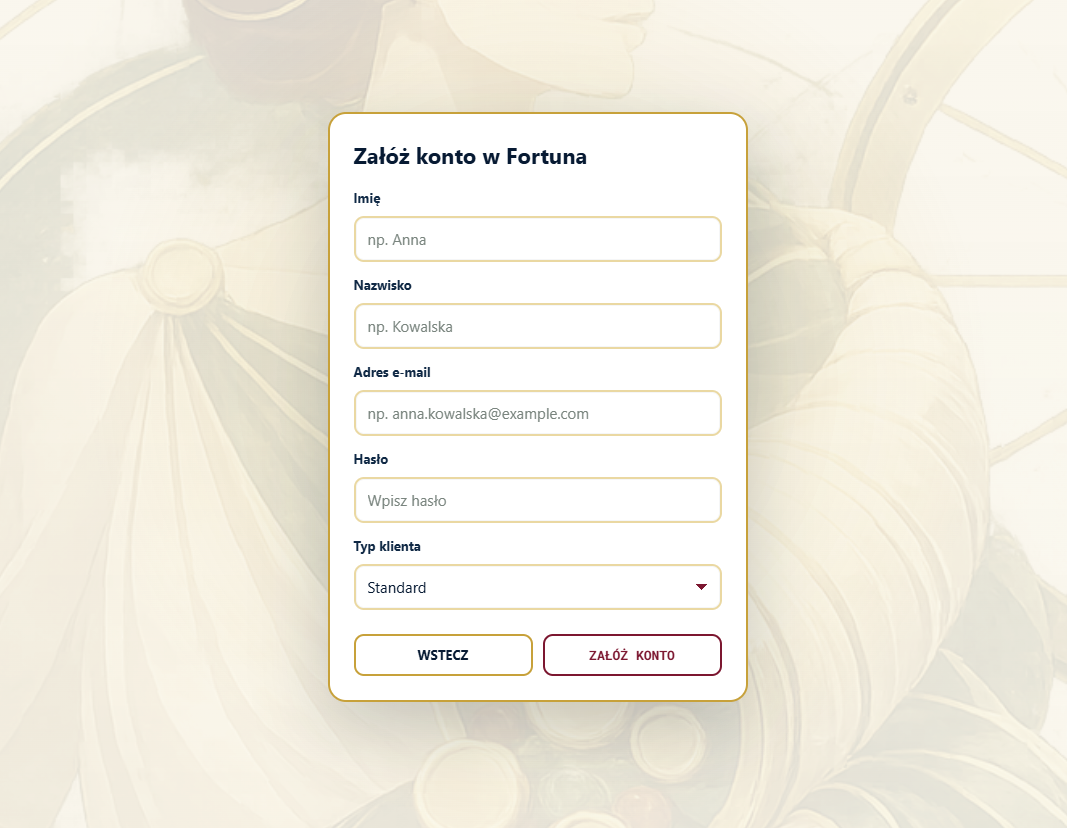
\includegraphics[width=0.68\textwidth]{creadte_account.png}
    \caption{Ekran rejestracji klienta.}
\end{figure}

\subsection{Logowanie}

Logowanie odbywa się przez endpoint \texttt{POST /api/customers/login}. W odpowiedzi API zwraca token JWT oraz datę wygaśnięcia. Token jest następnie dołączany w nagłówku \texttt{Authorization: Bearer ...} do żądań dashboardu i przelewów.

\begin{figure}[H]
    \centering
    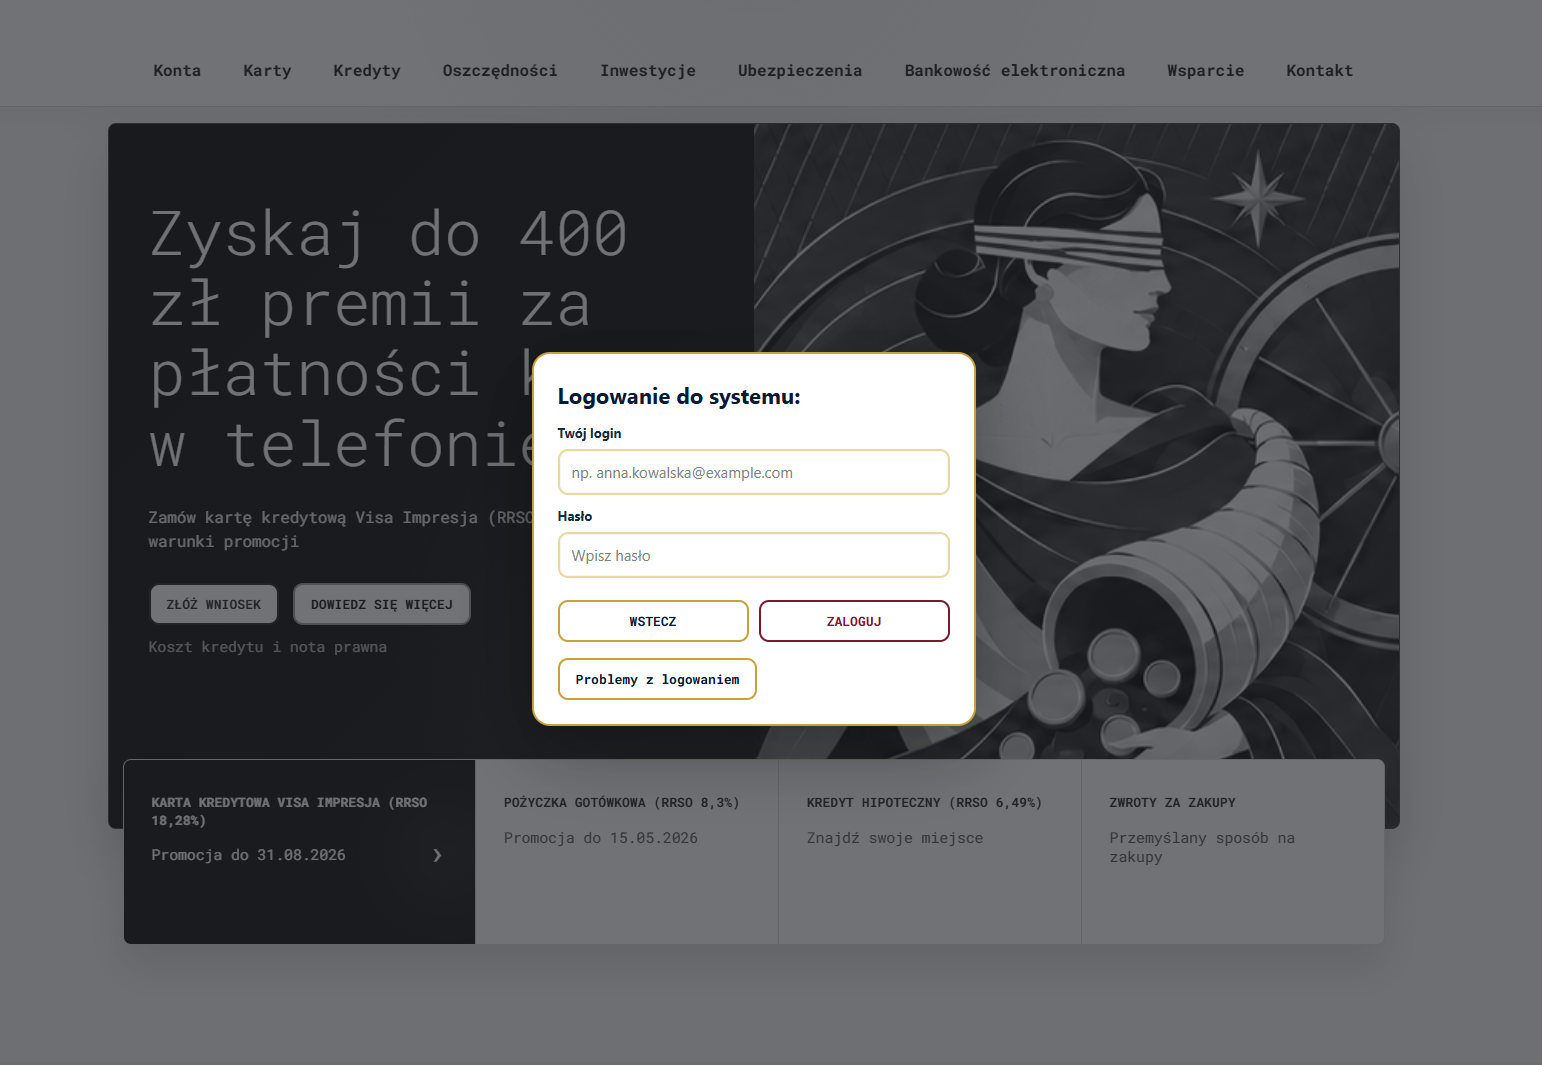
\includegraphics[width=0.55\textwidth]{logging.png}
    \caption{Popup logowania.}
\end{figure}

\subsection{Dashboard klienta}

Dashboard pokazuje łączną wartość środków, produkty klienta, skrót zdarzeń oraz akcje bankowe. Dane są pobierane z endpointu \texttt{GET /api/dashboard/\{customerId\}}, który korzysta z osobnego modelu odczytu.

\begin{figure}[H]
    \centering
    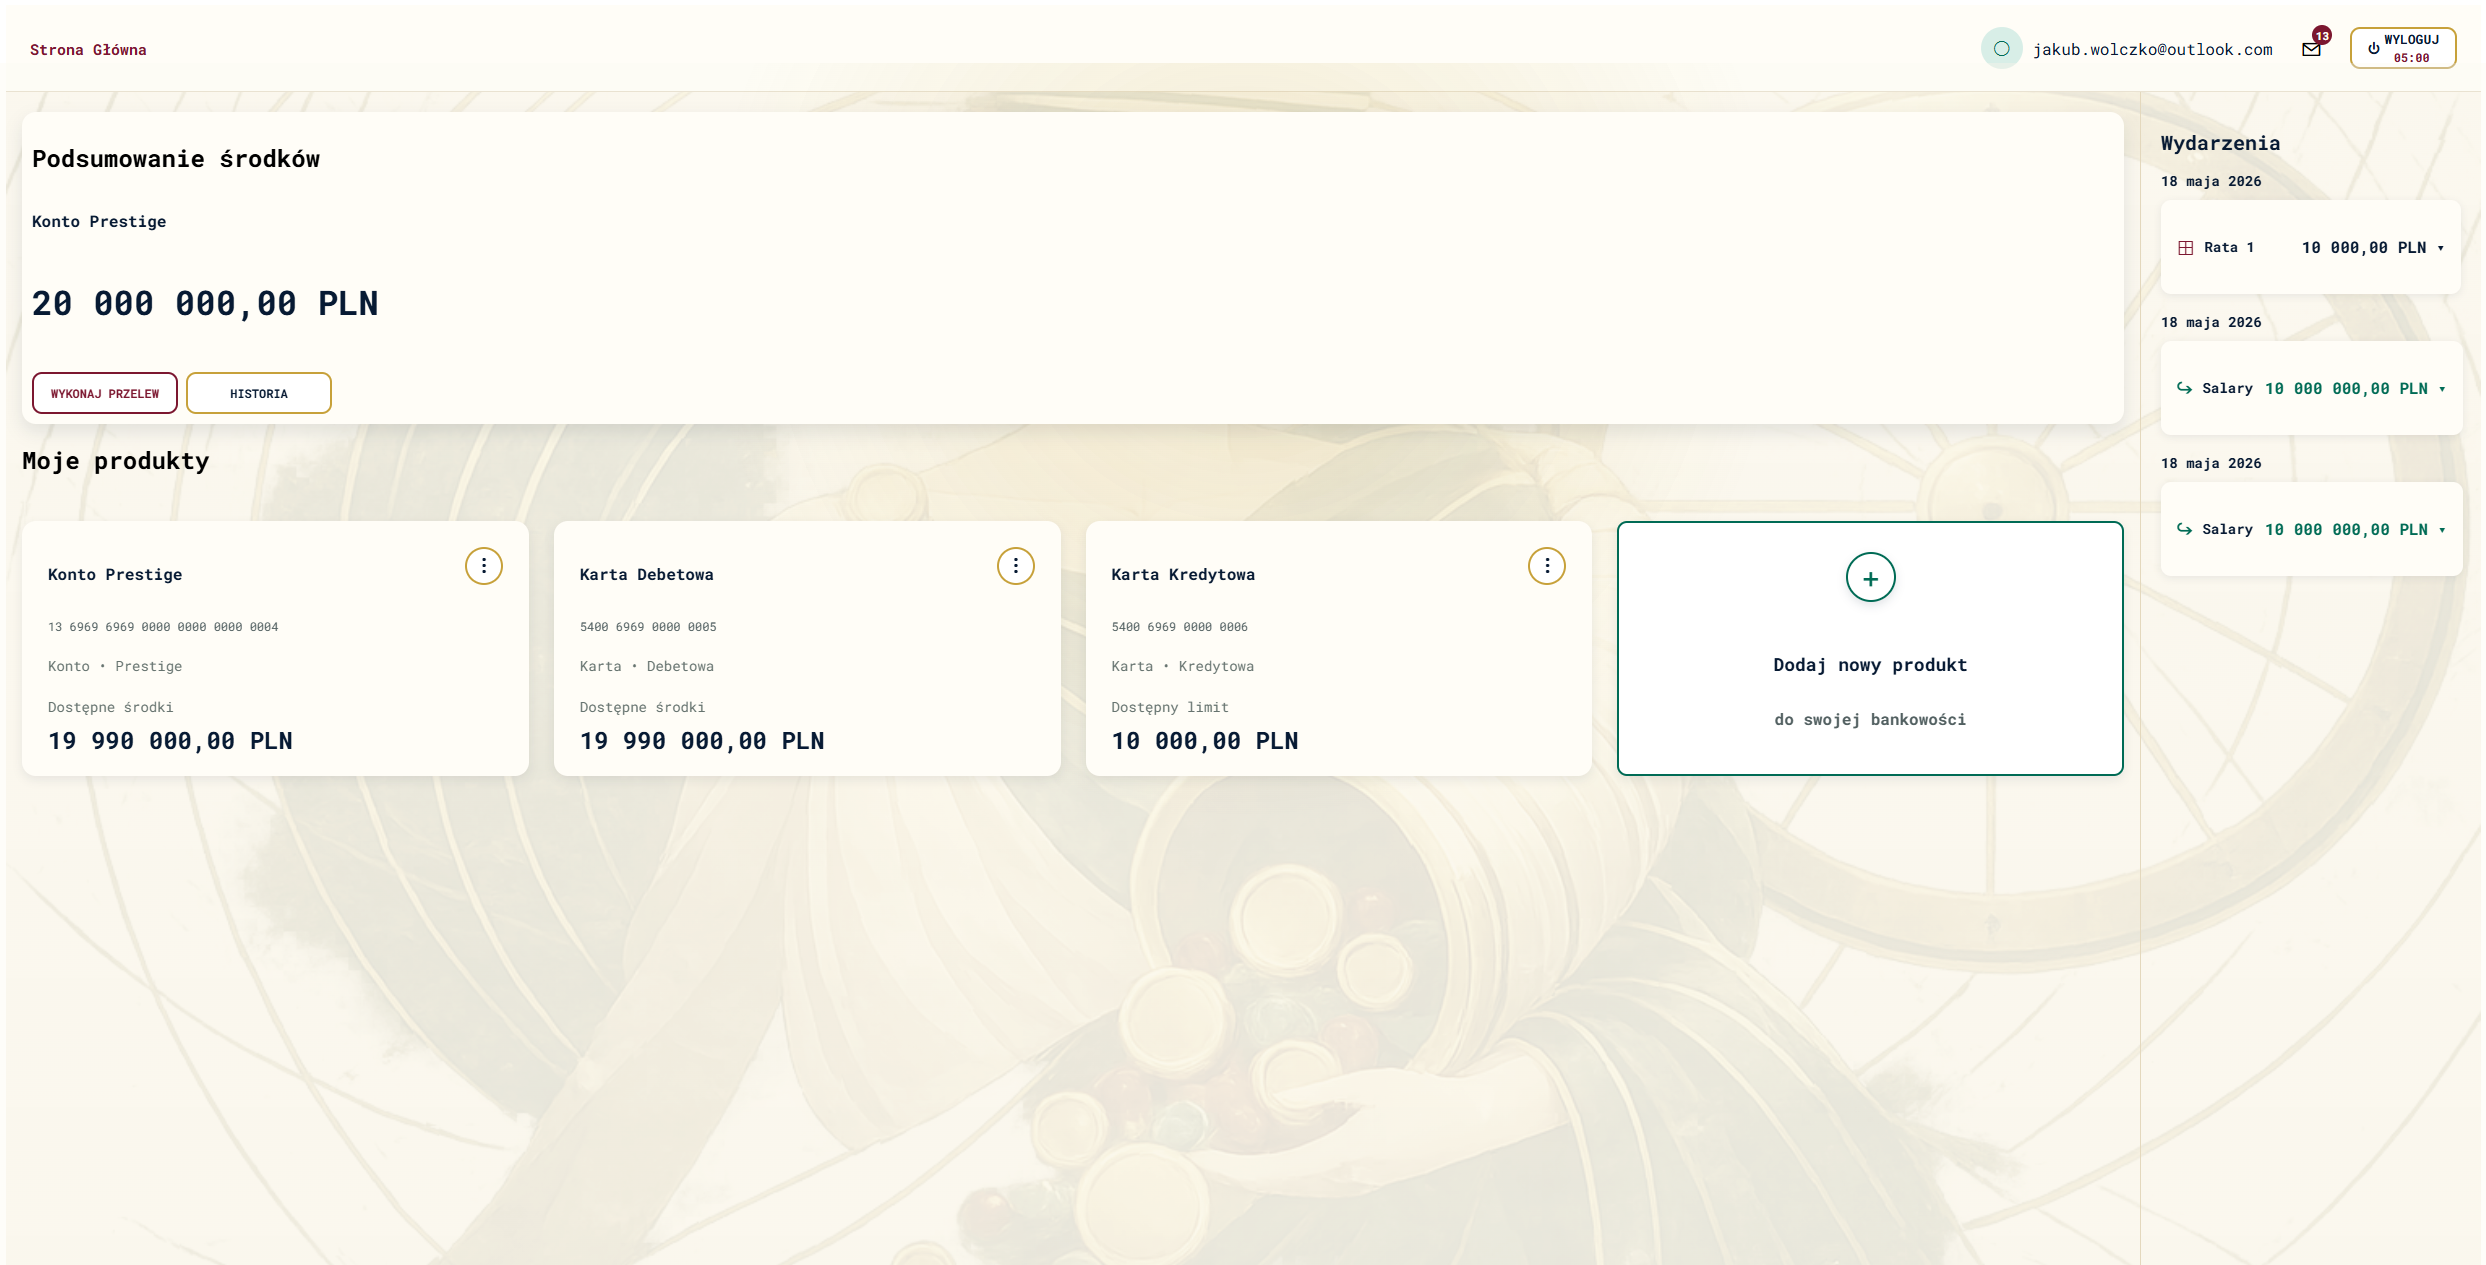
\includegraphics[width=0.95\textwidth]{dashboard.png}
    \caption{Dashboard klienta po zalogowaniu.}
\end{figure}

\subsection{Przelewy}

Popup przelewu pozwala wybrać typ przelewu, konto źródłowe, odbiorcę, tytuł i kwotę. Dla przelewów własnych wymagany jest produkt docelowy klienta, a dla przelewów zewnętrznych numer konta i nazwa odbiorcy.

\begin{figure}[H]
    \centering
    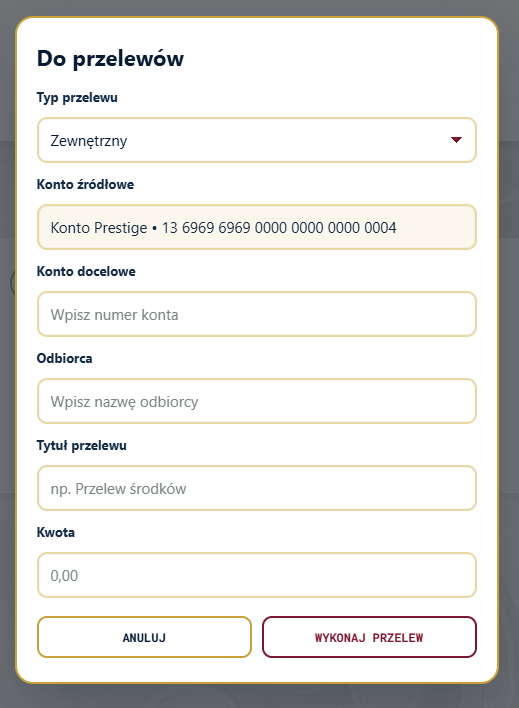
\includegraphics[width=0.55\textwidth]{przelewy.png}
    \caption{Formularz wykonywania przelewu.}
\end{figure}

\section{Architektura systemu}

System składa się z aplikacji frontendowej, backendu ASP.NET Core oraz dwóch logicznych modeli danych: zapisu i odczytu. Backend jest podzielony na projekty odpowiadające warstwom Clean Architecture.

\begin{figure}[H]
    \centering
    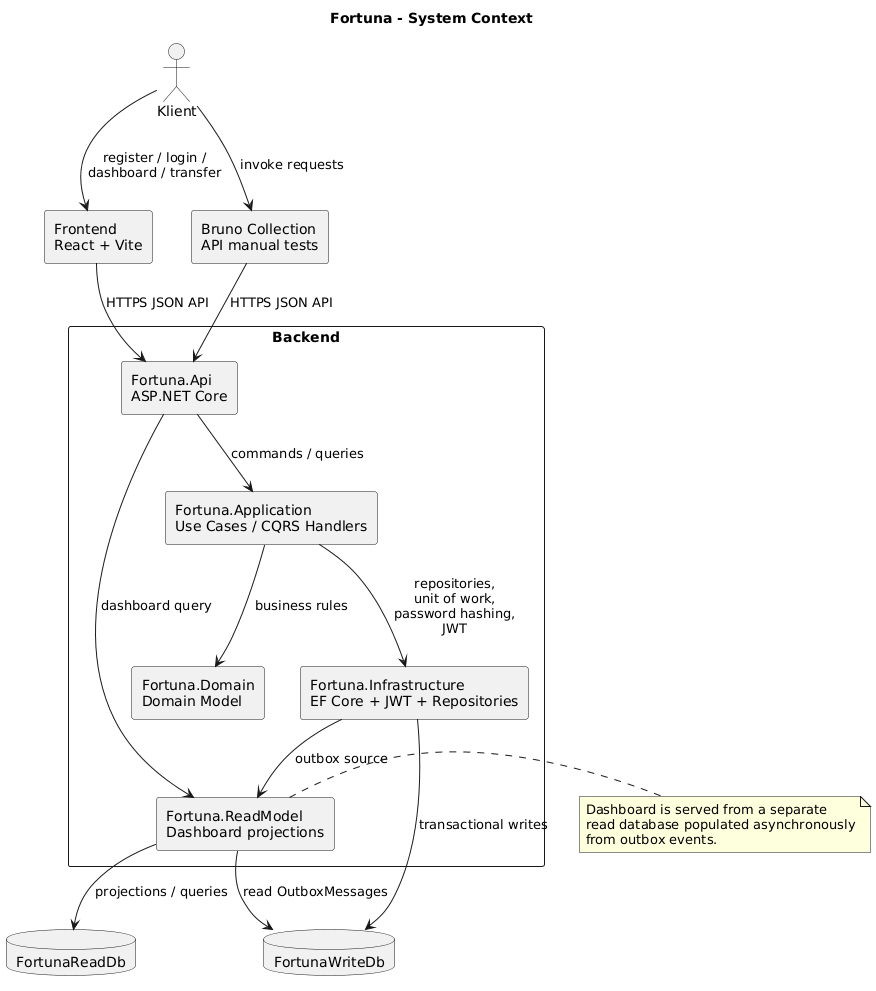
\includegraphics[width=0.9\textwidth]{system-context.png}
    \caption{Kontekst systemu Fortuna.}
\end{figure}

\subsection{Warstwy backendu}

\begin{longtable}{p{0.26\textwidth}p{0.66\textwidth}}
\toprule
\textbf{Projekt} & \textbf{Odpowiedzialność} \\
\midrule
\endhead
\texttt{Fortuna.Api} & Warstwa HTTP. Zawiera kontrolery, konfigurację CORS, Swagger, JWT, middleware obsługi wyjątków i mapowanie endpointów. \\
\texttt{Fortuna.Application} & Przypadki użycia systemu. Zawiera komendy, zapytania, handlery CQRS, abstrakcje repozytoriów, walidację scenariuszy i DTO dashboardu. \\
\texttt{Fortuna.Domain} & Model domenowy DDD: agregaty, encje, value objecty, reguły biznesowe i zdarzenia domenowe. \\
\texttt{Fortuna.Infrastructure} & Implementacje techniczne: EF Core dla bazy zapisu, repozytoria, Unit of Work, hashowanie haseł, JWT, Outbox processor. \\
\texttt{Fortuna.ReadModel} & Baza odczytu dashboardu, projekcje zdarzeń domenowych i repozytorium zapytań dashboardu. \\
\texttt{Fortuna.Contracts} & Kontrakty API używane przez kontrolery: requesty i response'y. \\
\bottomrule
\end{longtable}

\begin{figure}[H]
    \centering
    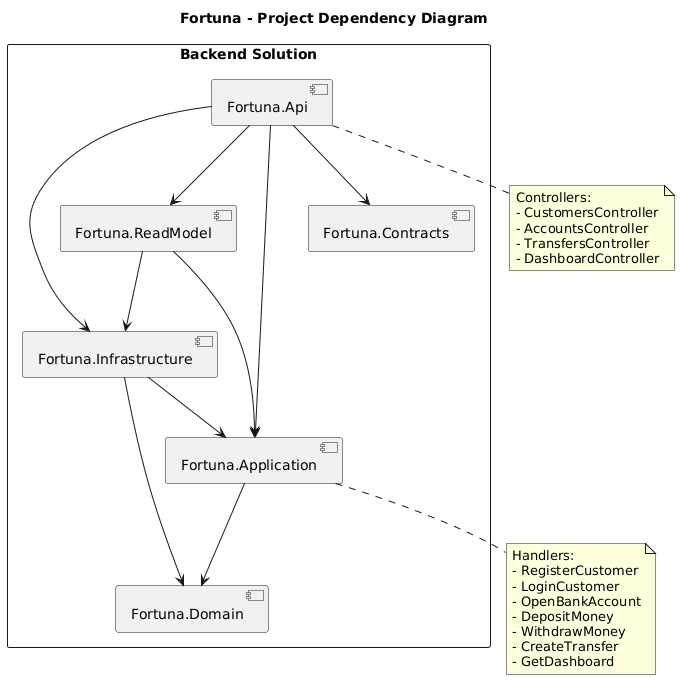
\includegraphics[width=0.8\textwidth]{backend-dependencies.png}
    \caption{Zależności projektów backendu.}
\end{figure}

Zależności są skierowane do wewnątrz. Warstwa domenowa nie zależy od infrastruktury ani API. Warstwa aplikacyjna zna domenę i abstrakcje, ale nie zna szczegółów EF Core czy JWT. Infrastruktura implementuje interfejsy wymagane przez Application.

\subsection{CQRS i rozdzielenie zapisu od odczytu}

Operacje zmieniające stan systemu są realizowane przez komendy, np. \texttt{RegisterCustomerCommand}, \texttt{CreateTransferCommand}, \texttt{DepositMoneyCommand}. Operacje odczytowe są realizowane przez zapytania, np. \texttt{GetDashboardQuery}.

Dashboard nie czyta bezpośrednio tabel transakcyjnych. Zamiast tego korzysta z bazy odczytu \texttt{FortunaReadDb}, która zawiera gotowe widoki danych: kafle produktów oraz zdarzenia osi czasu. Dzięki temu odczyt dashboardu jest prosty i szybki, a model zapisu może pozostać bliższy regułom domenowym.

\section{Model domenowy}

Główne pojęcia domenowe to klient, produkty finansowe, pieniądze, transakcje i przelewy. Produkty finansowe mają wspólną klasę bazową \texttt{Product}, po której dziedziczą \texttt{BankAccount}, \texttt{Card} i \texttt{Loan}. Klient jest właścicielem produktów, a konto lub karta mogą rejestrować operacje wpłat i wypłat.

\begin{figure}[H]
    \centering
    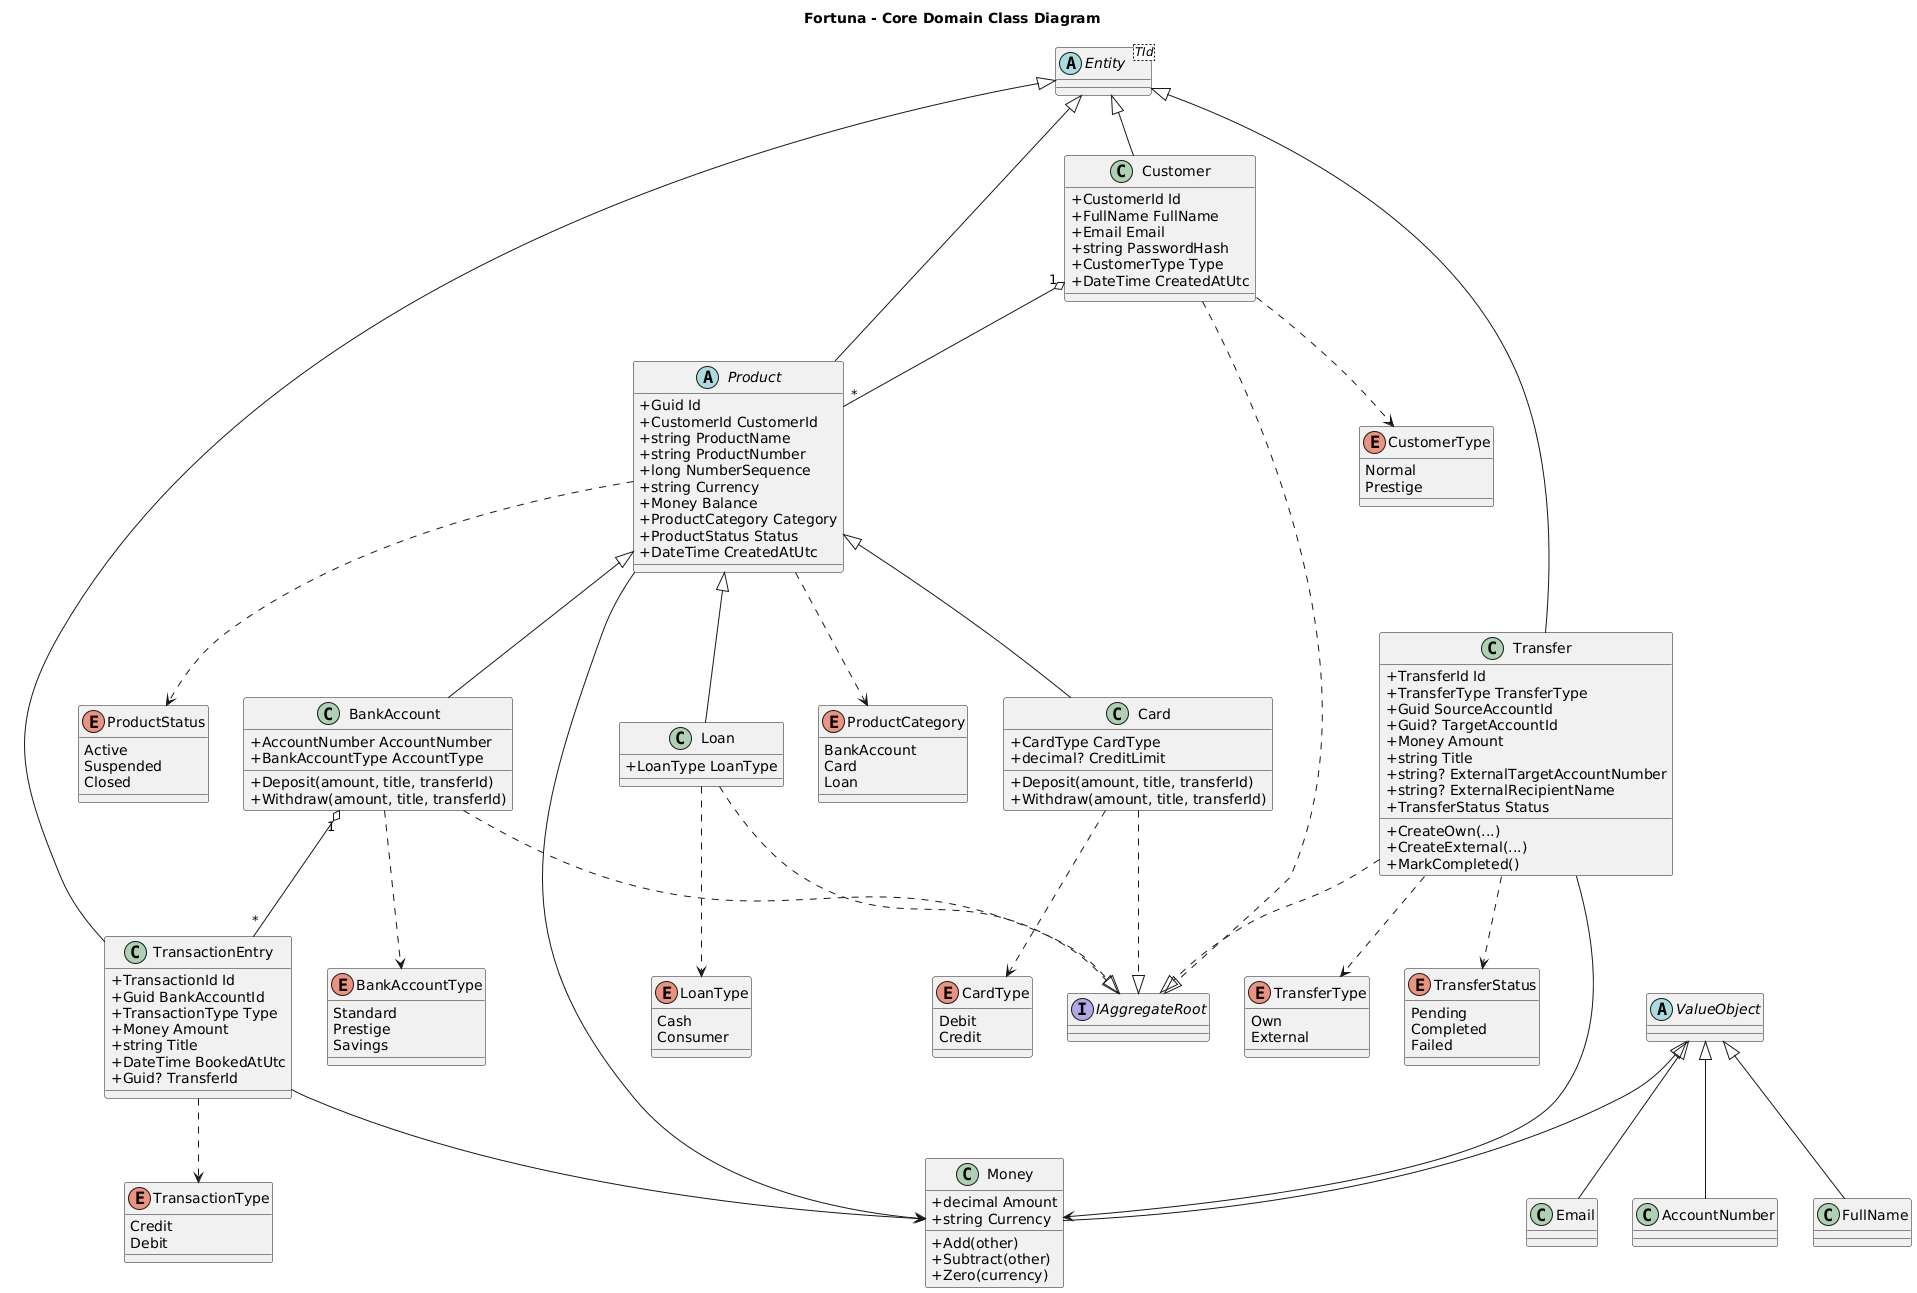
\includegraphics[width=0.95\textwidth]{domain-class-diagram.png}
    \caption{Diagram klas domenowych.}
\end{figure}

\subsection{Agregaty i value objecty}

Model używa podejścia DDD. Agregatami są między innymi \texttt{Customer}, \texttt{BankAccount}, \texttt{Card}, \texttt{Loan} i \texttt{Transfer}. Value objecty reprezentują dane z walidacją i znaczeniem domenowym, np. \texttt{Money}, \texttt{Email}, \texttt{FullName}, \texttt{AccountNumber}.

\begin{itemize}[nosep]
    \item \texttt{Money} przechowuje kwotę i walutę oraz udostępnia operacje dodawania i odejmowania.
    \item \texttt{Email} reprezentuje adres e-mail klienta i jest używany przy rejestracji oraz logowaniu.
    \item \texttt{FullName} rozdziela imię i nazwisko klienta.
    \item \texttt{AccountNumber} reprezentuje numer rachunku bankowego.
\end{itemize}

\subsection{Zdarzenia domenowe}

Encje domenowe generują zdarzenia, które są następnie zapisywane w tabeli \texttt{OutboxMessages}. Przykładowe zdarzenia to:
\begin{itemize}[nosep]
    \item \texttt{ProductCreatedDomainEvent},
    \item \texttt{MoneyDepositedDomainEvent},
    \item \texttt{MoneyWithdrawnDomainEvent},
    \item \texttt{TransferCreatedDomainEvent},
    \item \texttt{TransferCompletedDomainEvent}.
\end{itemize}

Zdarzenia są podstawą aktualizacji modelu odczytu.

\section{Działanie backendu}

\subsection{Rejestracja i logowanie}

Rejestracja jest obsługiwana przez \texttt{CustomersController} i \texttt{RegisterCustomerCommandHandler}. Handler sprawdza długość hasła, waliduje unikalność e-maila, hashuje hasło algorytmem PBKDF2 i zapisuje nowego klienta. Następnie tworzy produkty startowe:
\begin{itemize}[nosep]
    \item konto standardowe albo prestiżowe,
    \item kartę debetową,
    \item dodatkową kartę kredytową dla klienta typu Prestige.
\end{itemize}

Logowanie jest obsługiwane przez \texttt{LoginCustomerCommandHandler}. Handler pobiera klienta po adresie e-mail, sprawdza hasło i generuje token JWT. Token zawiera identyfikator klienta, który później służy do autoryzacji zapytań.

\begin{figure}[H]
    \centering
    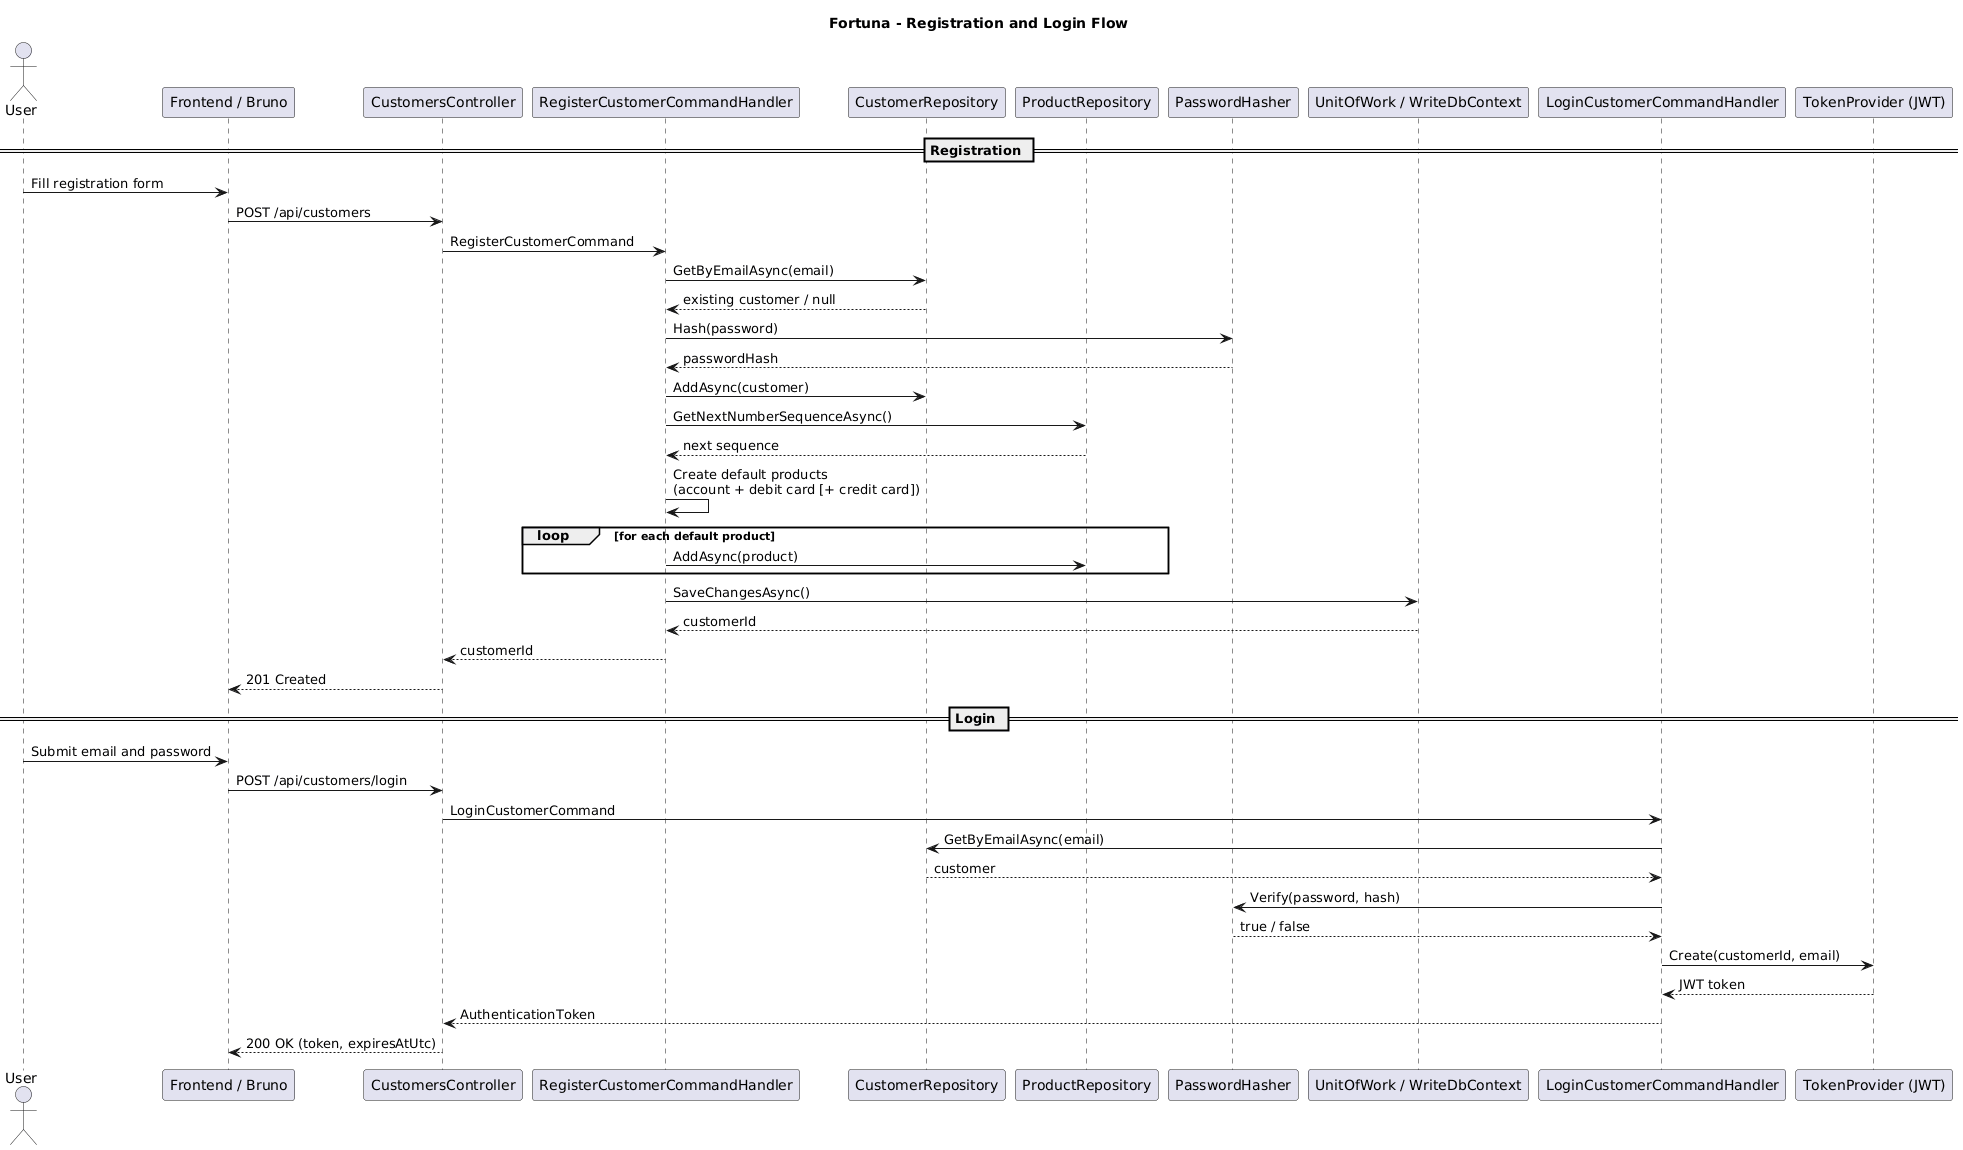
\includegraphics[width=0.95\textwidth]{registration-login-flow.png}
    \caption{Przepływ rejestracji i logowania.}
\end{figure}

\subsection{Pobieranie dashboardu}

Frontend wysyła żądanie \texttt{GET /api/dashboard/\{customerId\}} z tokenem JWT. Kontroler porównuje identyfikator z adresu URL z identyfikatorem zapisanym w tokenie. Jeśli identyfikatory są różne, zwracany jest \texttt{Forbid}. W przeciwnym razie \texttt{GetDashboardQueryHandler} pobiera dane z \texttt{DashboardReadRepository}.

\begin{figure}[H]
    \centering
    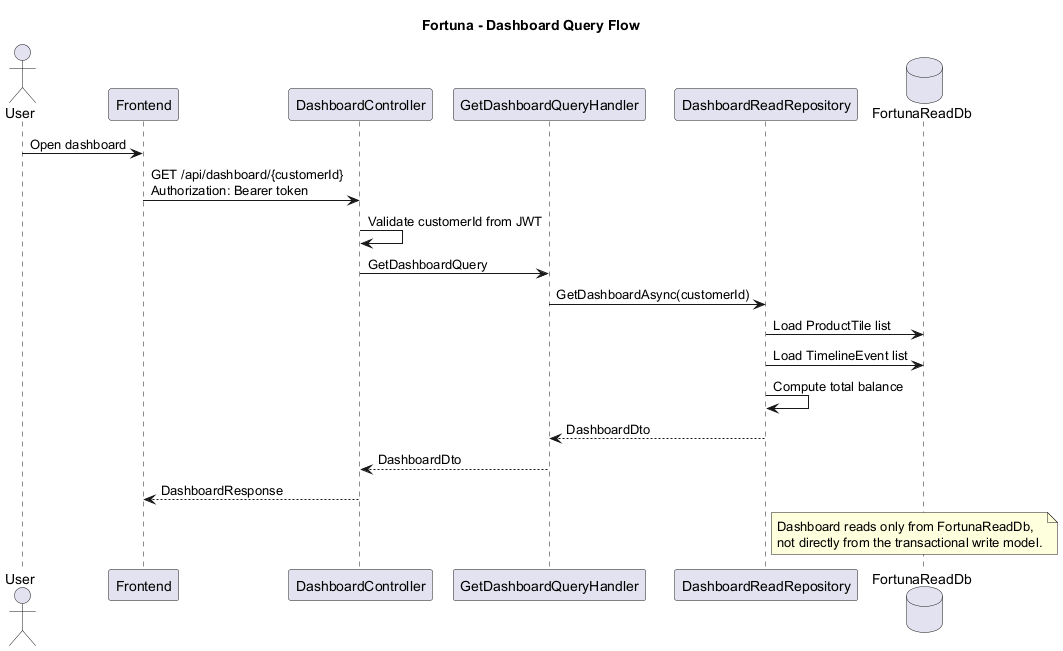
\includegraphics[width=0.95\textwidth]{dashboard-query-flow.png}
    \caption{Przepływ pobierania dashboardu.}
\end{figure}

\subsection{Wykonywanie przelewu}

Przelew jest obsługiwany przez \texttt{TransfersController} i \texttt{CreateTransferCommandHandler}. Handler odczytuje produkt źródłowy i sprawdza, czy należy do zalogowanego klienta. Następnie rozróżnia przelew własny i zewnętrzny.

Dla przelewu własnego system:
\begin{itemize}[nosep]
    \item pobiera produkt źródłowy i docelowy,
    \item sprawdza, czy oba należą do klienta,
    \item wykonuje wypłatę ze źródła,
    \item wykonuje wpłatę na cel,
    \item zapisuje przelew i oznacza go jako zakończony.
\end{itemize}

Dla przelewu zewnętrznego system:
\begin{itemize}[nosep]
    \item wymaga numeru rachunku odbiorcy i nazwy odbiorcy,
    \item wykonuje wypłatę z produktu źródłowego,
    \item zapisuje przelew zewnętrzny,
    \item oznacza przelew jako zakończony.
\end{itemize}

\begin{figure}[H]
    \centering
    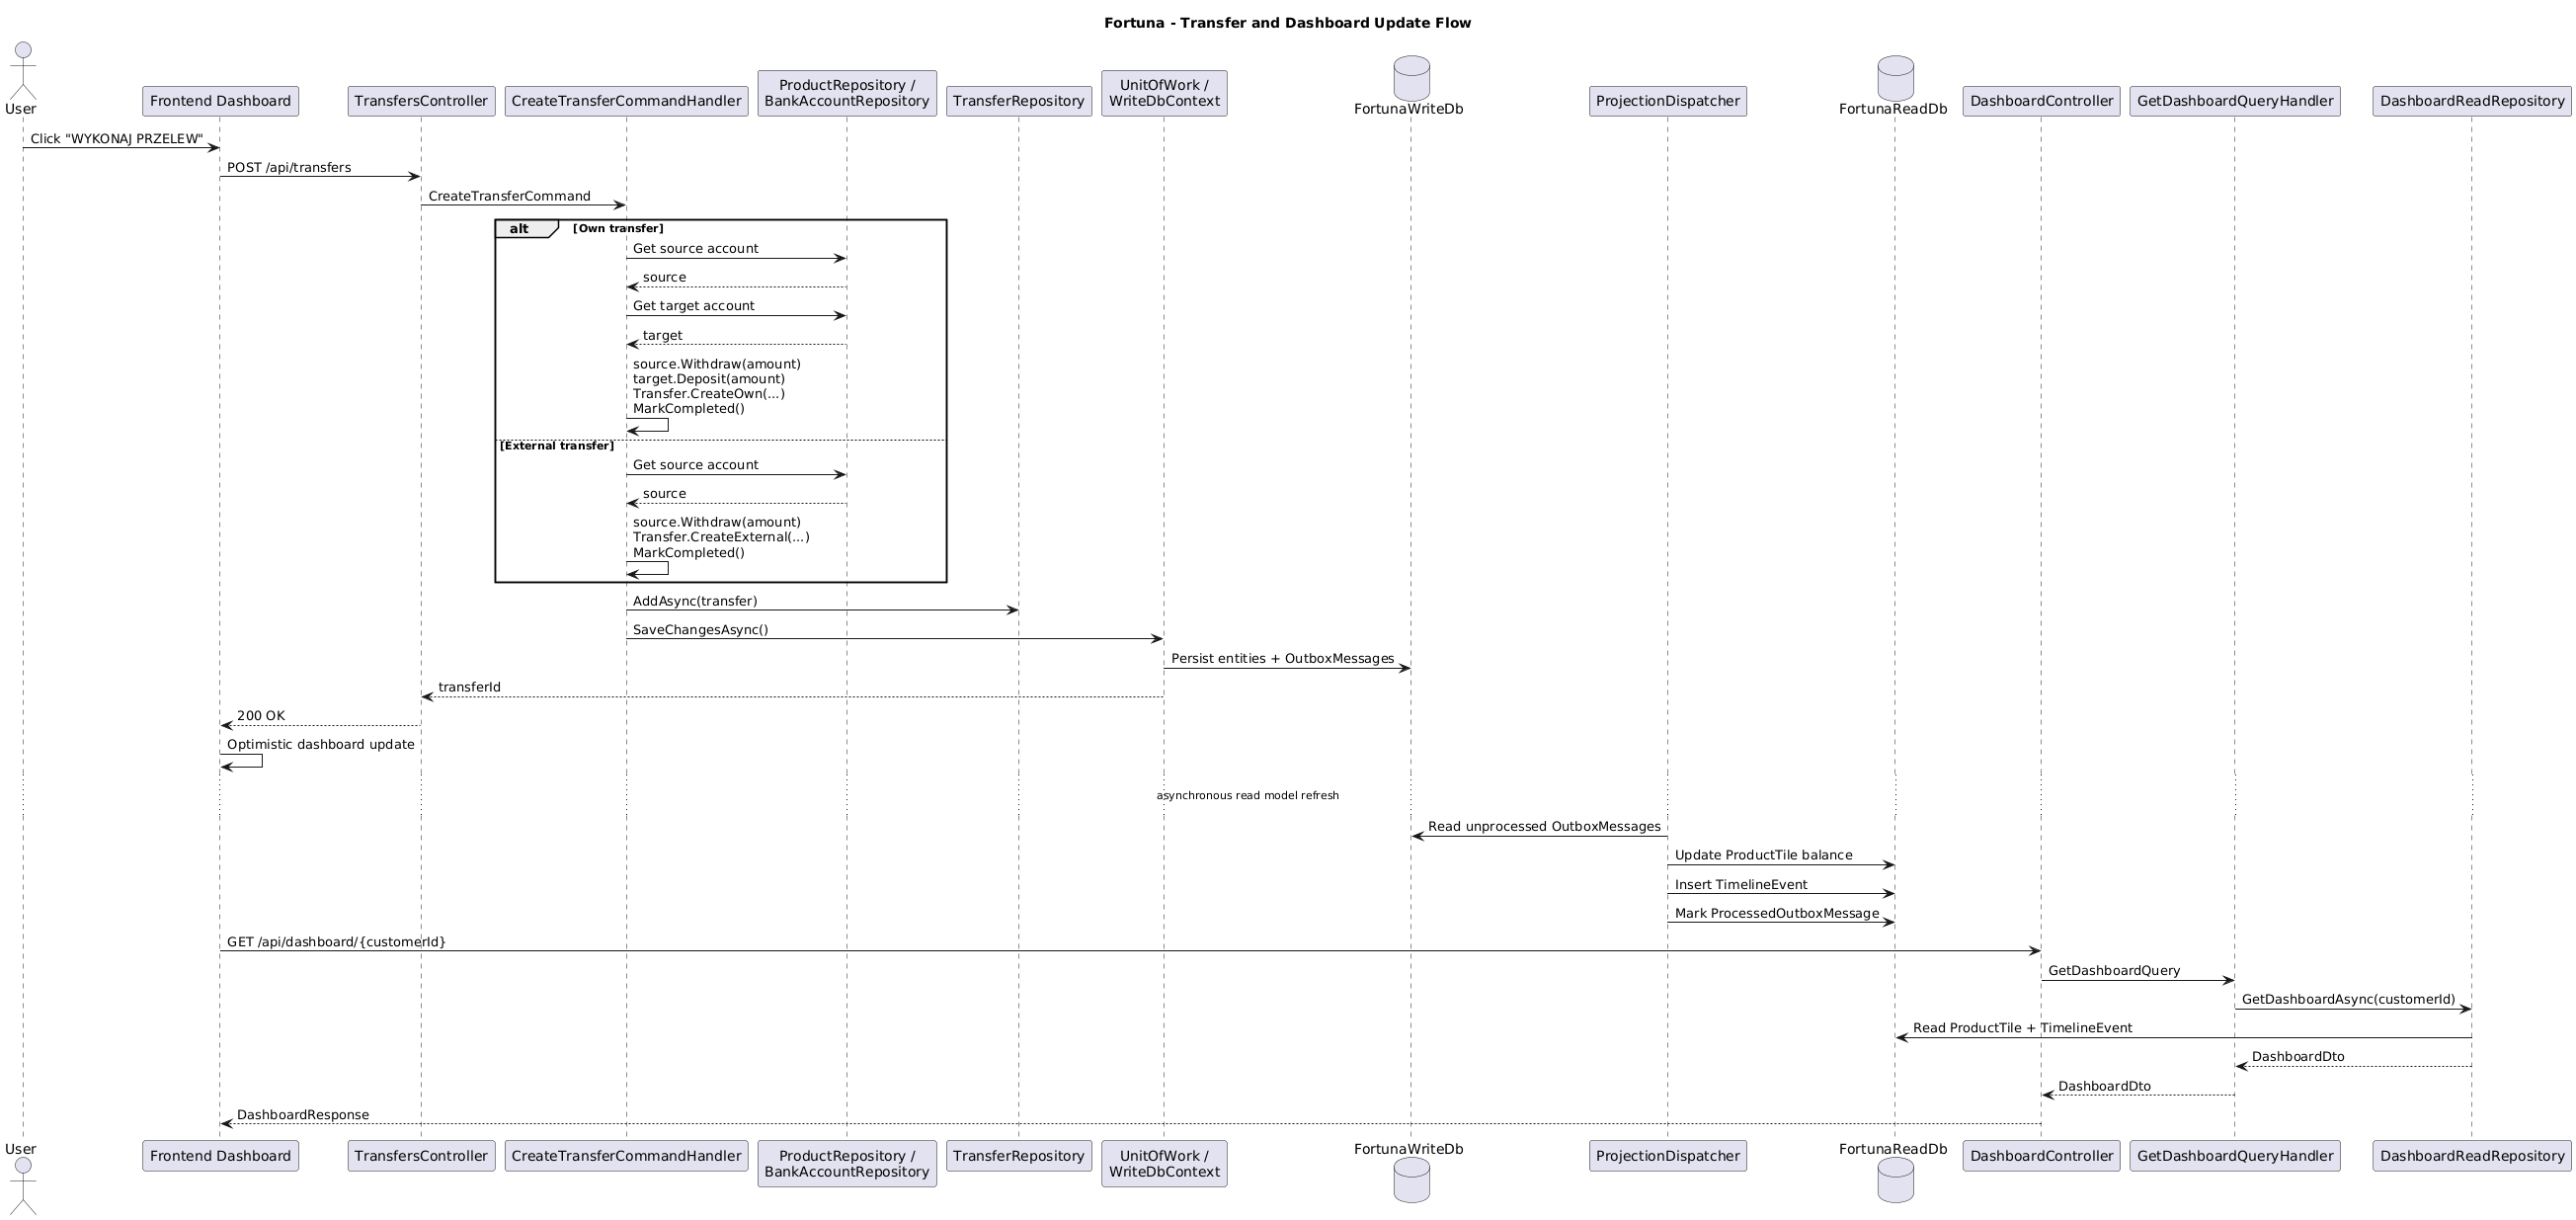
\includegraphics[width=0.95\textwidth]{transfer-dashboard-flow.png}
    \caption{Przelew i aktualizacja dashboardu.}
\end{figure}

\subsection{Symulacja przelewu przychodzącego}

Endpoint \texttt{POST /api/transfers/incoming} jest oznaczony jako \texttt{AllowAnonymous}. Służy do symulacji zewnętrznego wpływu środków, np. przy testowaniu przez Bruno. Komenda \texttt{DepositMoneyCommand} pobiera produkt docelowy, sprawdza, czy obsługuje wpłatę, zwiększa saldo i zapisuje zmiany.

\begin{figure}[H]
    \centering
    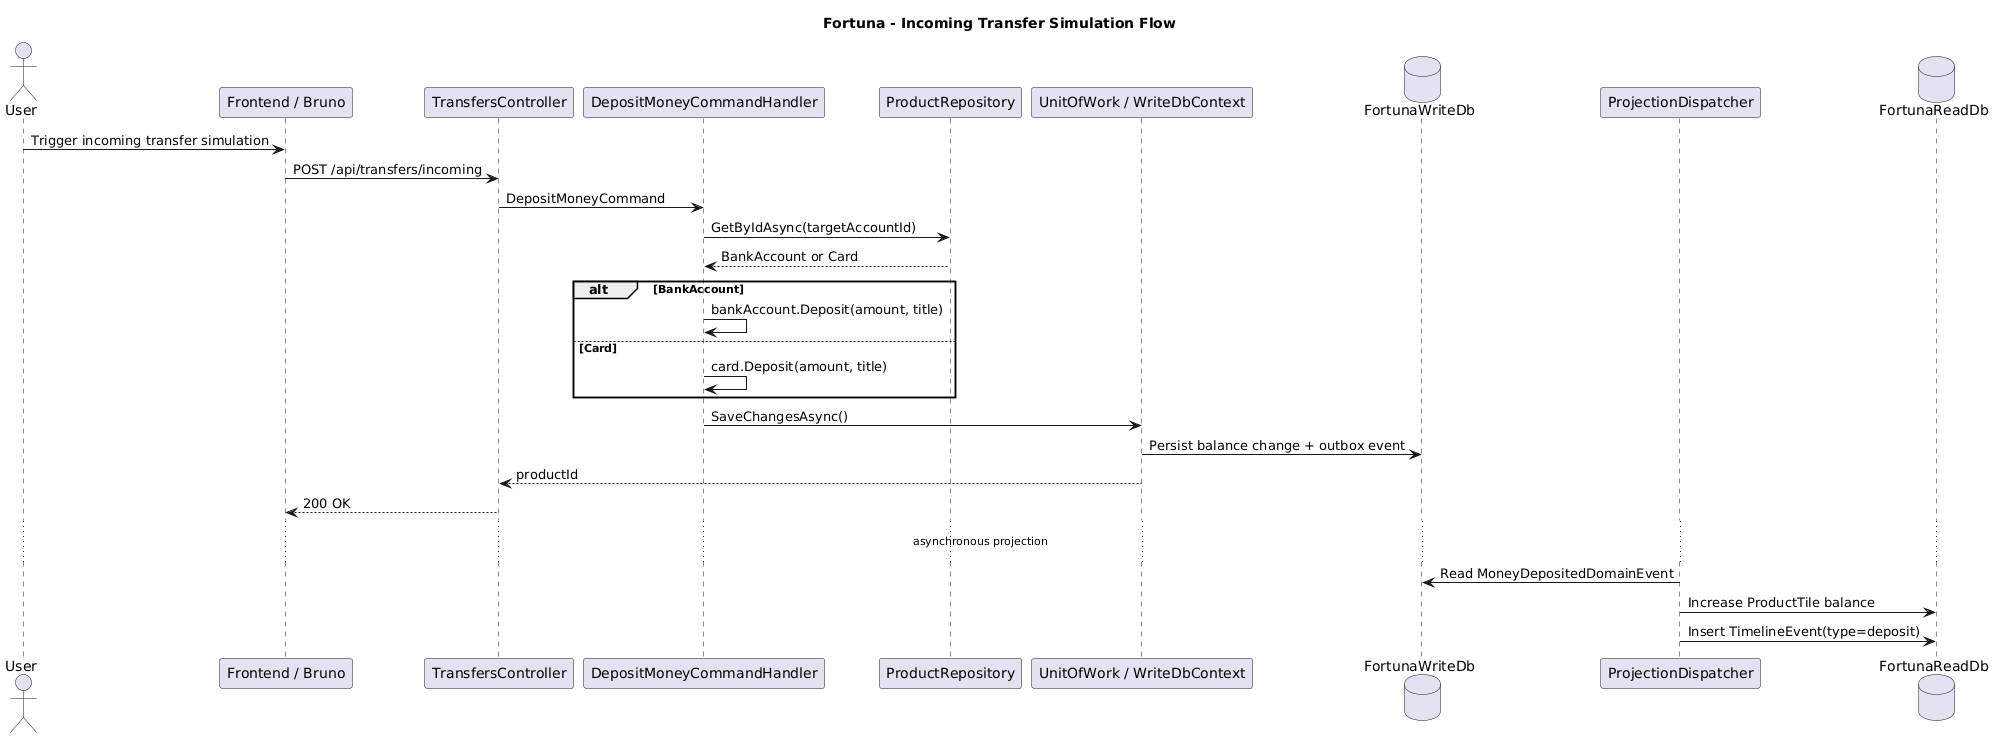
\includegraphics[width=0.95\textwidth]{incoming-transfer-flow.png}
    \caption{Symulacja przelewu przychodzącego.}
\end{figure}

\section{Mechanizm Outbox i projekcje}

Podczas \texttt{SaveChangesAsync} w \texttt{WriteDbContext} system przegląda encje posiadające zdarzenia domenowe. Każde zdarzenie jest serializowane do JSON i zapisywane jako rekord w tabeli \texttt{OutboxMessages}. Po zapisaniu zmian zdarzenia są czyszczone z encji.

Proces w tle \texttt{OutboxMessageProcessor} cyklicznie pobiera nieprzetworzone wiadomości z bazy zapisu. Dla każdej wiadomości wywoływany jest \texttt{ProjectionDispatcher}, który aktualizuje bazę odczytu. Po poprawnym przetworzeniu rekord w \texttt{OutboxMessages} otrzymuje \texttt{ProcessedOnUtc}, a w bazie odczytu zapisywany jest wpis \texttt{ProcessedOutboxMessage}.

Projekcje obsługują między innymi:
\begin{itemize}[nosep]
    \item utworzenie kafla produktu po \texttt{ProductCreatedDomainEvent},
    \item zwiększenie salda i dodanie zdarzenia osi czasu po \texttt{MoneyDepositedDomainEvent},
    \item zmniejszenie salda i dodanie zdarzenia osi czasu po \texttt{MoneyWithdrawnDomainEvent}.
\end{itemize}

\section{Schematy baz danych}

System używa dwóch logicznych baz danych SQL Server: bazy zapisu \texttt{FortunaWriteDb} i bazy odczytu \texttt{FortunaReadDb}. Schemat jest pokazany na diagramie ERD.

\begin{figure}[H]
    \centering
    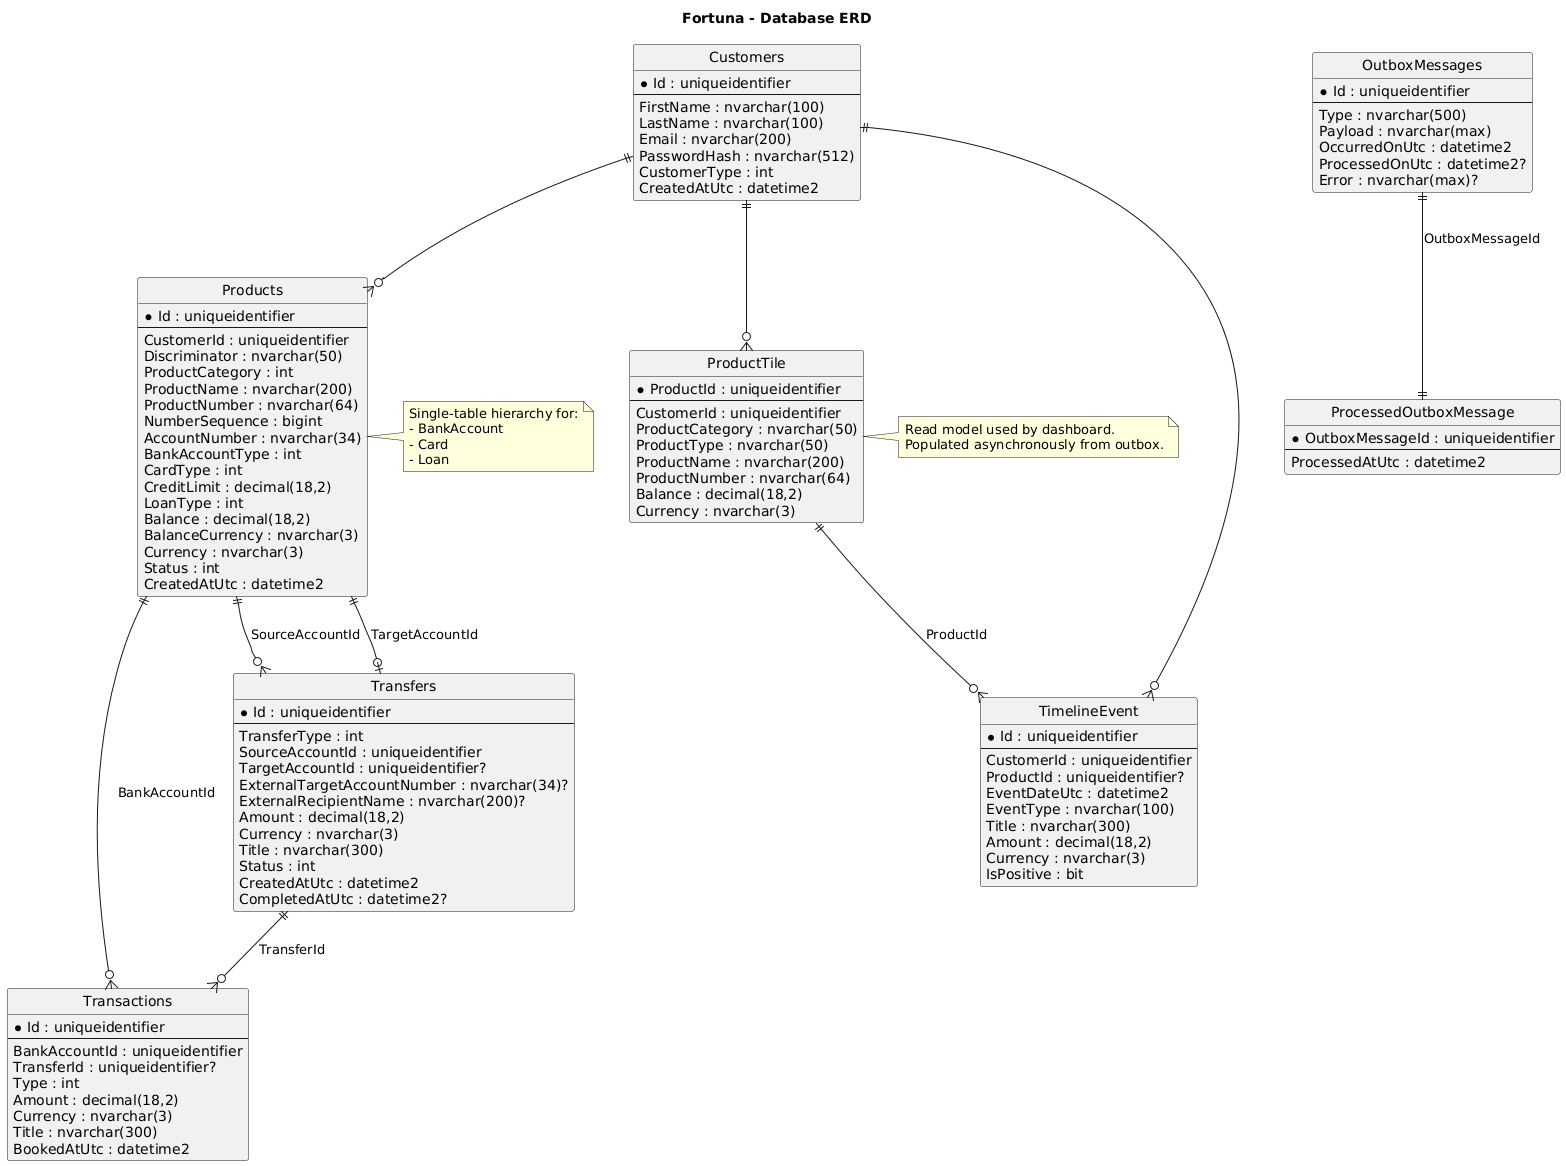
\includegraphics[width=0.95\textwidth]{database-erd.png}
    \caption{Diagram ERD baz danych.}
\end{figure}

\subsection{Baza zapisu}

Baza zapisu przechowuje stan transakcyjny systemu i jest zarządzana przez \texttt{WriteDbContext}. To ona jest źródłem prawdy dla operacji domenowych.

\begin{longtable}{p{0.23\textwidth}p{0.67\textwidth}}
\toprule
\textbf{Tabela} & \textbf{Opis} \\
\midrule
\endhead
\texttt{Customers} & Dane klientów: identyfikator, imię, nazwisko, e-mail, hash hasła, typ klienta i data utworzenia. E-mail jest unikalny. \\
\texttt{Products} & Wspólna tabela dla produktów finansowych. EF Core używa dziedziczenia typu single-table hierarchy z kolumną \texttt{Discriminator}. W tabeli znajdują się konta, karty i kredyty. \\
\texttt{Transactions} & Zapisy księgowe dla wpłat i wypłat. Zawierają produkt, typ transakcji, kwotę, walutę, tytuł, datę księgowania i opcjonalny identyfikator przelewu. \\
\texttt{Transfers} & Przelewy własne i zewnętrzne. Zawierają źródło, opcjonalny cel wewnętrzny, dane odbiorcy zewnętrznego, kwotę, status oraz daty utworzenia i zakończenia. \\
\texttt{OutboxMessages} & Zserializowane zdarzenia domenowe oczekujące na projekcję do bazy odczytu. \\
\bottomrule
\end{longtable}

\subsection{Baza odczytu}

Baza odczytu jest zoptymalizowana pod dashboard. Nie odtwarza pełnego modelu domenowego, tylko gotowe struktury potrzebne do wyświetlenia interfejsu.

\begin{longtable}{p{0.28\textwidth}p{0.62\textwidth}}
\toprule
\textbf{Tabela} & \textbf{Opis} \\
\midrule
\endhead
\texttt{ProductTile} & Kafle produktów widoczne na dashboardzie. Zawiera produkt, klienta, kategorię, typ, nazwę, numer, saldo i walutę. \\
\texttt{TimelineEvent} & Zdarzenia widoczne w panelu aktywności. Zawiera klienta, opcjonalny produkt, datę, typ zdarzenia, tytuł, kwotę, walutę i informację, czy zdarzenie zwiększa saldo. \\
\texttt{ProcessedOutboxMessage} & Identyfikatory wiadomości Outbox już przetworzonych przez projekcje. Chroni przed wielokrotnym przetworzeniem tego samego zdarzenia. \\
\bottomrule
\end{longtable}

\subsection{Najważniejsze relacje}

\begin{itemize}[nosep]
    \item Jeden klient ma wiele produktów.
    \item Produkt typu konto bankowe może mieć wiele transakcji.
    \item Przelew ma produkt źródłowy i opcjonalny produkt docelowy.
    \item Transakcja może być powiązana z przelewem.
    \item Jeden klient ma wiele kafli produktu i zdarzeń osi czasu w modelu odczytu.
    \item Rekord Outbox może odpowiadać jednemu rekordowi \texttt{ProcessedOutboxMessage}.
\end{itemize}

\section{Frontend}

Frontend znajduje się w katalogu \texttt{frontend/src}. Aplikacja używa React Router do routingu, Redux Toolkit do stanu autoryzacji oraz TanStack Query do pobierania danych dashboardu.

\subsection{Struktura}

\begin{longtable}{p{0.25\textwidth}p{0.65\textwidth}}
\toprule
\textbf{Katalog} & \textbf{Opis} \\
\midrule
\endhead
\texttt{app} & Konfiguracja routera, klient API, providery i store Redux. \\
\texttt{features/auth} & Logowanie, rejestracja, sesja użytkownika i slice autoryzacji. \\
\texttt{features/dashboard} & Pobieranie danych dashboardu, typy i prezentacja produktów. \\
\texttt{features/transfers} & API przelewów, typy formularza i lokalna aktualizacja dashboardu po przelewie. \\
\texttt{components} & Komponenty widoków: landing page, logowanie, rejestracja, dashboard i przelewy. \\
\texttt{views} & Komponenty stron routingu: landing, login, create account, dashboard. \\
\texttt{shared/ui} & Wspólne komponenty UI, np. Button, Input, InfoPopup. \\
\bottomrule
\end{longtable}

\subsection{Komunikacja z API}

Frontend używa funkcji \texttt{apiRequest}. Rejestracja i logowanie wysyłają żądania anonimowe. Dashboard i przelewy dodają nagłówek \texttt{Authorization}. Po wykonaniu przelewu frontend wykonuje lokalną, optymistyczną aktualizację danych, a następnie może pobrać odświeżony dashboard z read modelu.

\section{Bezpieczeństwo i walidacja}

Backend używa JWT Bearer Authentication. Endpointy kont, dashboardu i przelewów wymagają zalogowania. Kontroler dashboardu dodatkowo sprawdza, czy klient próbuje pobrać własne dane, porównując identyfikator z URL z identyfikatorem z tokenu.

Hasła nie są przechowywane jawnie. Implementacja \texttt{Pbkdf2PasswordHasher} zapisuje hash hasła. Rejestracja wymaga hasła o długości co najmniej 8 znaków, a logowanie zwraca błąd autoryzacji dla niepoprawnego e-maila albo hasła.

Walidacja reguł biznesowych znajduje się w handlerach i modelu domenowym. Przykładowo przelew zewnętrzny wymaga numeru rachunku i nazwy odbiorcy, przelew własny wymaga innego produktu docelowego niż źródłowy, a operacje wpłat i wypłat są obsługiwane tylko dla kont oraz kart.

\section{Podsumowanie}

Fortuna jest aplikacją wielowarstwową, w której frontend React komunikuje się z backendem ASP.NET Core przez REST API. Backend realizuje Clean Architecture i DDD, a przypadki użycia są rozdzielone zgodnie z CQRS. Model zapisu przechowuje pełny stan domenowy i generuje zdarzenia, natomiast osobny model odczytu udostępnia dane zoptymalizowane dla dashboardu. Mechanizm Outbox zapewnia asynchroniczne i kontrolowane przenoszenie zmian z modelu zapisu do modelu odczytu.

\end{document}
